% Como fue implementando, interesa la implementaci\'on m\'as que el algoritmo gen\'erico,
%  es decir, si se tiene que implementar SA, lo que se espera es que se explique en pseudo
%  codigo la estructura general y en parrafo explicativo cada parte como fue implementada
%  para su caso particular, si se utilizan oparadores se debe explicar por que se utilizo

%  ese operador, si fuera el caso de una t\'ecnica completa, si se utiliza recursi\'on o no,
%  etc. En este punto no se espera que se incluya codigo, eso va aparte.
El algoritmo utilizado para resolver el \emph{Car Sequencing Problem (CSP)} fue un
\emph{Algoritmo Evolutivo} con mutación \emph{Simulated Annealing}.

Las siguientes sub-secciones describen con más detalle como se adaptó la teoría de
los presentes algoritmos para resolver el \emph{CSP}.

\subsection{Población Inicial}
Una de las cosas mas importantes a la hora de evaluar si una solución es viable o no,
es su factibilidad, es decir, si cumple con todas las \emph{restricciones duras}.

Para solucionar lo anterior es que al momento de crear \emph{la población inicial},
se realizó de una forma aleatoria, pero cumpliendo con todas las \emph{restricciones
duras}, es decir, generando sólo \emph{restricciones factibles}.

Primero que todo se generó una secuencia ordenada con la cantidad de tipos de autos
requerida, es decir, si tuviéramos las siguientes demandas:
\begin{itemize}
	\item Tipo 1: 2 autos.
	\item Tipo 2: 1 auto.
	\item Tipo 3: 3 autos.
	\item Tipo 4: 6 autos.
\end{itemize}
La secuencia generada sería:

$$1\ 1\ 2\ 3\ 3\ 3\ 4\ 4\ 4\ 4\ 4\ 4$$

Una vez tengamos la secuencia, procedemos a generar todos los individuos de nuestra población
inicial, lo cual se realizó, desordenando la secuencia anterior, de una forma aleatoria.

% conclusión
Si nos damos cuenta, la forma de generar nuestra población, quizás no es la más adecuada
debido a que se generó de manera aleatoria, pero al generar solo soluciones factibles,
estamos mejorando mucho más éste aspecto, sin embargo, la utilización de  una técnica para
la construcción de soluciones iniciales, podría mejorar el performance de nuestro algoritmo,
por ejemplo si utilizáramos una técnica \emph{Greedy} o \emph{GRASP}.

\subsection{Evaluación de la población}

Para realizar la evaluación de una determinada población, se tiene en cuenta lo siguiente:

Es necesario recorrer toda la población, luego, una vez seleccionado un individuo, se procede
a recorrer mediante subsecuencias (de tamaño establecido en el problema, $sizeMaxOptCarSeq$)
todo el individuo (serie de autos), y por cada iteración vamos verificando si se cumplen las
restricciones blandas, es decir, sumamos la cantidad de autos con una opción determinada y
luego verificamos si esa suma es menor o igual al máximo permitido por las restricciones ($numMaxOptCarSeq$).

Si por cada suma en cada subsecuencia, no se cumple la restricción, se le asigna un \emph{fitness}
equivalente a las unidades por las cuales se excede el máximo establecido, al individuo en cuestión.

Finalmente, si encontramos alguna restricción factible que posea un \emph{fitness} igual a $0$,
inmediatamente, nos quedamos con dicha solución y el algoritmo termina.

\subsection{Selección de Individuos}

Al momento de seleccionar un individuo para realizar una transformación, se utilizó la conocida técnica llamada
\emph{roulette wheel}, para una Función Objetivo que minimiza.

El procedimiento es bien simple, sólo tenemos que considerar el \emph{fitness} de cada individuo y calcular un
\emph{fitness relativo} de la siguiente forma:

$$relativeFitness_{i}\ = \frac{f_{min} + f_{max} - f_{i}}{\sum\limits_{i=0}^{sizePop} (f_{min} + f_{max} - f_{i}}$$

Donde $f_{max}$ equivale al \emph{fitness} del mejor individuo,
$f_{min}$ equivale al \emph{fitness} del peor individuo y 
$f_{i}$ equivale al \emph{fitness} del i-ésimo individuo de nuestra población.

La suma de todos los \emph{fitness relativo} equivale a $1$.

Luego de que cada individuo posee su \emph{fitness relativo}, se procede a calcular un \emph{fitness acumulativo},
es decir, ir sumando las probabilidades para generar un rango entre $0$ y $1$ con todas nuestras probabilidades.

Una vez se tiene el \emph{fitness acumulativo} listo, se procede a obtener un número aleatorio entre $0$ y $1$,
para que luego sea ubicado en nuestro rango, y así el individuo que salga escogido con éste número aleatorio, será
elegido para pasar ahora a la transformación.

El siguiente ejemplo, ayuda a la comprensión del presente procedimiento:\\

\begin{minipage}{0.2\textwidth}
	\begin{tabular}{|r|r|}
	\hline
	\textbf{individuo} & \textbf{Fitness} \\ \hline
	1 & 50 \\\hline
	2 & 30 \\\hline
	3 & 20 \\\hline
	\end{tabular}
\end{minipage}
\  \ 
\hfill \begin{minipage}{0.2\linewidth}
	Tenemos ahora:
	\begin{itemize}
		\item $f_{min}$: 20
		\item $f_{max}$: 50
	\end{itemize}
\end{minipage}
\  \
\hfill \begin{minipage}{0.35\textwidth}
	\vspace{0.4cm}
	\begin{itemize}
		\item $f_{min}\ +\ f_{max}$: 70
		\item $\sum\limits_{i=1}^{3} (f_{min} + f_{max} - f_{i})$: 110
	\end{itemize}
\end{minipage}\\


Ahora procedemos a calcular el fitness relativo y acumulativo:\\

\begin{center}
\begin{tabular}{|r|r|r|r|}
\hline
\textbf{individuo} & \textbf{Fitness} & \textbf{Fitness relativo} & \textbf{Fitness acumulativo}\\ \hline
1 & 50 & 0.18 & 0.18 \\\hline
2 & 30 & 0.36 & 0.54 \\\hline
3 & 20 & 0.46 & 1.00 \\\hline
\end{tabular}
\end{center}

\begin{figure}[htb!]
	\begin{center}
	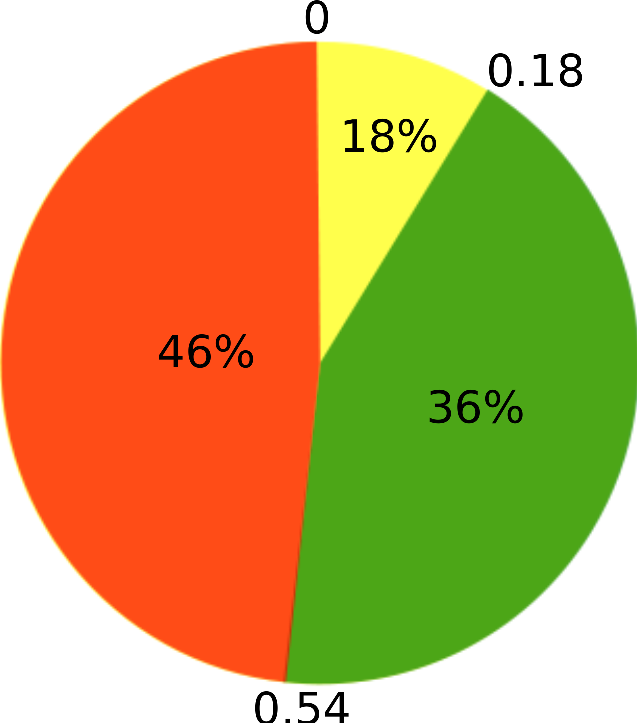
\includegraphics[scale=0.4]{img/fig1}
	\end{center}
	\label{fig:fig1}
	\caption{Gr\'afico final mediante el método de la ruleta}
\end{figure}

Si ahora escogiéramos un número aleatorio entre $0$ y $1$, por ejemplo $0.6$, tenemos que mirar la \textbf{Figura 1} de la sección~\ref{fig:fig1} y caeríamos
en el lugar del individuo 3, por lo que él sería escogido.

De esta forma, se les da una probabilidad a cada individuo para poder pasar a la nueva población, dependiendo
netamente de que tan bueno sea.

Este proceso se repite hasta que tenemos a todos los individuos de nuestra población nueva.


\subsection{Transformación de Individuos}

Por lo general, en las implementaciones de transformación, existe tanto la \emph{mutación} como el \emph{cruzamiento},
de los cuales, ambos poseen una cierta probabilidad asociada, para que cuando se escoja un individuo, se obtiene
un número aleatorio entre $0$ y $1$ y si ese número es menor o igual que la probabilidad de mutación, se muta,
lo mismo ocurre con el cruzamiento.

\subsubsection{Mutación}
Según los requerimientos del problema, la mutación debe ser la técnica \emph{Simulated Annealing} y se escogió la variación
de \emph{Alguna Mejora}, para obtener un menor tiempo de ejecución.

Pasos de la implementación:

\begin{itemize}
	\item Paso 0: Inicialización.
	\begin{itemize}
		\item X := solución inicial factible
		\item tmax := máximo número de iteraciones (IMAX)
		\item q := temperatura alta inicial (TMAX)
		\item Mejor solución := X
		\item Número de iteraciones = t := 0
	\end{itemize}
	\item Paso 1: Parada.
	\begin{itemize}
		\item Si la cantidad de iteraciones mayor a tmax o si la temperatura es menor que $0$,
			entonces paramos.
		\item Entregar mejor solución.
	\end{itemize}
	\item Paso 2: Movimiento.
	\begin{itemize}
		\item Realizamos el movimiento, en éste caso se realiza un \emph{swap},
			pero como cada individuo es del orden de $200$, $300$ y $400$ autos,
			se realiza una cantidad de \emph{swap} equivalente al $10\%$ de la cantidad de autos.
			
			Para ver que elementos hacen el \emph{swap}, se eligen aleatoriamente dos elementos para intercambiar.
		\item Calculamos la disminución de la FO (Dobj).
	\end{itemize}
	\item Paso 3: Aceptación.
	\begin{itemize}
		\item Si X(t+1) mejor el objetivo ó
		\item Si $e^{\frac{-Dobj}{q}}\ \ge\ random(0,1)$ entonces
		\item X(t+1) := X(t), sino
		\item volver al Paso 2.
		
	\end{itemize}
	\item Paso 4: Reemplazar el mejor.
	\begin{itemize}
		\item Si el valor de la FO de X(t+1) es mejor a la Mejor Solución, entonces:
		\item Mejor solución := X(t+1)
	\end{itemize}
	\item Paso 5: Reducción de la temperatura.
	\begin{itemize}
		\item Si han pasado 3 iteraciones desde el último cambio de temperatura, reducimos q a un $90\%$.
		\item q := q * 0.9.
	\end{itemize}
	\item Paso 6: Incrementar.
	\begin{itemize}
		\item t := t + 1, Volver al Paso 1. 
	\end{itemize}
\end{itemize}

Una vez terminada la mutación, se pasa el individuo (Mejor solución) a la siguiente población.

\subsubsection{Cruzamiento}
Por el lado del cruzamiento, la presente implementación no lo posee, debido a la \emph{representación} del problema.
La técnica escogida fue \emph{cruzamiento en un punto}, pero no se realizó, debido a que rompería las restricciones duras
del problema, y nos generaría individuos que serían soluciones infactibles.\\

A continuación se señala un diagrama explicativo:
Consideremos las siguientes demandas por 3 tipos de autos.\\

\begin{minipage}{0.2\textwidth}
	\begin{itemize}
		\item Tipo 1: 3
		\item Tipo 2: 1
		\item Tipo 3: 2
	\end{itemize}
\end{minipage}
\  \  
\hfill\begin{minipage}{0.4\textwidth}
	\begin{itemize}
		\item Padre 1: 3 2 1 1 3 1
		\item Padre 2: 1 3 3 2 1 1
	\end{itemize}
\end{minipage}

\begin{figure}[htb!]
	\begin{center}
	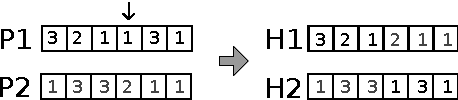
\includegraphics[scale=1]{img/fig2}
	\end{center}
	\label{fig:fig2}
	\caption{Explicación de violación de restricciones duras por cruzamiento}
\end{figure}

En la \textbf{Figura 2} de la sección~\ref{fig:fig2} podemos darnos cuenta que no estamos respetando las restricciones
duras de la cantidad de autos de Tipo 2 y 3, entonces si nos damos cuenta de que éste es un ejemplo
pequeño, la cantidad de restricciones violadas con una mayor cantidad de autos, será mucho mayor.

Como en el caso de los algoritmos evolutivos, el cruzamiento se encarga de explotar,
la explotación es suplida por la mutación \emph{Simulated Annealing}, ya que como bien sabemos,
a temperaturas altas, explora y a temperaturas bajas, explota.

\subsection{Elitismo}

Para la presente implementación, se consideró el elitismo como una pieza fundamental para poder
mejorar nuestra nuevas poblaciones.

Una vez que tengamos una población, el elitismo se encarga de buscar el individuo con más alto \emph{fitness},
y se reemplaza con el individuo que tenga el fitness más bajo, además siempre el mejor individuo de cada población
pasa directamente a la siguiente población, con lo cual se asegura no perder soluciones buenas con el pasar
de las poblaciones.

\subsection{Estructura del Algoritmo}

Tomando en cuenta toda la descripción anterior,
el algoritmo central sería:

\begin{verbatim}
	Inicio
	g <- 0 // numero de generaciones
	p <- 0 // numero de poblaciones
	Leer datos de entrada
    Población <- Generar población inicial
    Evaluar población

	    Mientras g < GENS
			Mientras n < POP - 1
				Selección individuo
				Mutación // Simulated Annealing + AM 
			Fin Mientras
			Elitismo
			Cambio de población // Población actual = Población nueva
			Evaluar población
	        n <- n + 1
	        p <- 0
		Fin Mientras
	Imprimir resultados
	Fin
\end{verbatim}

\subsection{Parámetros}

Para la presente implementación, se trabajó con una seria de constantes definidas antes de la ejecución del algoritmo,
las cuales fueron variadas para observar el desempeño del algoritmo, dejando las más apropiadas:
\begin{description}
	\item[VARS]: Número de variables (autos) de la secuencia, el cual es cambiado para cada experimento ($200$, $300$ y $400$).
	\item[POP]:  Tamaño de cada población.
	\item[GENS]: Número de generaciones.
	\item[PMUT]: Probabilidad de mutación. Se considero de que como no se realiza cruzamiento, la presente probabilidad se aumentó.
	\item[TMAX]: Temperatura Máxima para el \emph{Simulated Annealing}.
	\item[IMAX]: Número máximo de iteraciones para el \emph{Simulated Annealing}.
\end{description}
